\section{3D空间的线性变换}

	在MVS任务中要着重研究各个相机成像平面之间的变换关系,下面是3D空间到自身的一些变换(2D空间也类似)。\\

	变换的本质是探究在某些变换群下,那些不变的性质,所以下面每个变换都探讨什么不变,所用的都是其次坐标。

	\subsection{欧式变换}
		对目标进行平移和旋转,保持目标大小、长度、夹角都不变。表示矩阵为,
		$$
			H_E = \begin{bmatrix}
				\mathbf{R}_{3\times 3}\quad& \mathbf{t}_{3\times 1}\\
				0_{1\times 3} \quad& 1_{1\times 1}
			\end{bmatrix}
		$$

		$R$是$3\times 3$的旋转矩阵,$t$是平移向量。\\

		可以验证虚圆点是$H_E$的两个特征向量。这说明欧式变换的本质是虚圆点不变,大小、长度、夹角都是因为虚圆点不变而成立。\\

		\textit{2D欧式变换有3个自由度,3D的有6个自由度}

	\subsection{相似变换}
		均匀缩放的欧式变换,目标大小、长度发生变化,但夹角不变,
		$$
			H_S = \begin{bmatrix}
				s\mathbf{R}_{3\times 3}\quad& \mathbf{t}_{3\times 1}\\
				0_{1\times 3} \quad& 1_{1\times 1}
			\end{bmatrix}
		$$

		$s$是缩放尺度,3个方向上相同。可以验证,虚圆点也是相似变换的特征向量。\\

		\textit{2D相似变换有4个自由度,3D的有7个自由度}
	
	\subsection{仿射变换}
		非均匀缩放的欧式变换,夹角不能保持,但能保持平行线变换后仍为平行,无穷远平面不变。
		$$
			H_A = \begin{bmatrix}
				\mathbf{A}_{3\times 3}\quad& \mathbf{t}_{3\times 1}\\
				0_{1\times 3} \quad& 1_{1\times 1}
			\end{bmatrix}
		$$

		$A$是一个可逆矩阵。\\

		标准无穷远平面$\pi_{\infty} = (0,0,0,1)^T$,根据点面对偶原理,平面变换为,
		\begin{align*}
			\pi_{\infty}^{\prime} = H_A^{-T}\pi_{\infty} 
			&=
			\begin{bmatrix}
				\mathbf{A}_{3\times 3}\quad& \mathbf{t}_{3\times 1}\\
				0_{1\times 3} \quad& 1_{1\times 1}
			\end{bmatrix}^{-T}
			\begin{bmatrix}
				\mathbf{0}_{3\times 1}\\
				1
			\end{bmatrix}\\
			&=
			\begin{bmatrix}
				\mathbf{A}^{-T}\quad& \mathbf{0}\\
				-\mathbf{t}^TA^{-T} \quad& 1
			\end{bmatrix}
			\begin{bmatrix}
				\mathbf{0}\\
				1
			\end{bmatrix}\\
			&= (0,0,0,1)^T\\
			&=\pi_{\infty} 
		\end{align*}

		容易验证,$l_{\infty}, \pi_{\infty}$是仿射映射的特征向量。\\

		仿射变换可分解为(以2D为例),
		$$
			\mathbf{A} = \mathbf{R}(\theta)\mathbf{R}(-\phi)
			\begin{pmatrix}
				s_x \quad &0\\
				0 \quad & s_y
			\end{pmatrix}
			\mathbf{R}(\phi)
		$$

		$s_x,s_y$为在$x,y$方向的放缩因子,$\theta,\phi$为旋转角度,如此可以看出仿射变换的确是非均匀缩放的欧式变换。\\

		\textit{2D仿射变换有6个自由度,3D的有12个自由度}
	
	\subsection{射影变换}

		\textbf{射影变换} 又称为 \textbf{单应变换},这两个名字会混着用。\\

		对非奇异$\mathbf{H}$,变换$x^\prime = \mathbf{H}x + \mathbf{b}$;若$\mathbf{b} = 0$,则为射影变换;否则不是。\\

		变换矩阵具有更一般的形式,平行性和无穷远平面也保持不了,但能保持线性性,即直线仍映射为直线。
		$$
			H_P = \begin{bmatrix}
				\mathbf{A}_{3\times 3}\quad& \mathbf{t}_{3\times 1}\\
				\mathbf{v}_{1\times 3} \quad& 1_{1\times 1}
			\end{bmatrix}
		$$

		以2D为例,对直行$x^Tl = 0$,变换后的点$x^\prime = H_Px$,变换后的$l^\prime = H_P^{-T}l$,

		$$
			x^\prime l^\prime = \left(H_Px\right)^TH_P^{-T}l = x^T H_P^TH_P^{-T}l = 0
		$$

		2D空间中的确直线变为直线。3D空间的直线表示比较复杂,需用两个平面交线表示:$x^T\pi_A =0,  x^T\pi_B =0$,
		\begin{align*}		
			x^\prime \pi_A^{\prime} &= (H_Px)^T(H_P^{-T}\pi_A) = x^TH_P^TH_P^{-T}\pi_A = 0\\
			x^\prime \pi_B^{\prime} &= (H_Px)^T(H_P^{-T}\pi_B) = x^TH_P^TH_P^{-T}\pi_B = 0
		\end{align*}

		所以3D空间的线性性也得到保证。如下情况会存在平面间的射影变换,

		\begin{itemize}
			\item 场景如果是平面,则场景平面与像平面间的变换
			\item 场景是平面,则不同相机的成像平面之间的变换
			\item 同一相机,只有旋转没有平移拍摄到的像平面之间的变换;这种拍摄方式常用来做广角图拼接
			\item 同一光心透视两张平面之间形成的变换
		\end{itemize}

		如果场景不是平面,则不同相机像平面之间一般不是射影变换,通过极几何约束这种对应关系。\\

		射影变换可以进行层次化分解,$\mathbf{H} = \mathbf{H_S}\mathbf{H_A}\mathbf{H_P}$,
		$$
			\begin{pmatrix}
				\mathbf{A}_{3\times 3}\quad& \mathbf{t}_{3\times 1}\\
				\mathbf{v}_{1\times 3} \quad& 1_{1\times 1}
			\end{pmatrix}
			=
			\begin{pmatrix}
				s\mathbf{R}_{3\times 3}\quad & \mathbf{t}_{3\times 1}\\
				\mathbf{0}_{1\times 3}\quad & 1_{1\times 1}
			\end{pmatrix}
			\begin{pmatrix}
				\mathbf{K}_{3\times 3}\quad & \mathbf{0}_{3\times 1}\\
				\mathbf{0}_{1\times 3}\quad & 1_{1\times 1}
			\end{pmatrix}
			\begin{pmatrix}
				\mathbf{I}_{3\times 3}\quad & \mathbf{0}_{3\times 1}\\
				\mathbf{v}_{1\times 3}\quad & 1_{1\times 1}
			\end{pmatrix}
		$$
		\textit{2D透视变换有7个自由度,3D的有15个自由度}
	\subsection{仿射恢复}

		仿射变换使得无穷远点保持不变,而射影变换则使得无穷远点变为有限点,如下图\footnote{\url{https://www.graphicsmill.com/docs/gm/affine-and-projective-transformations.htm}},

		\begin{figure}[H]
			% \begin{center}
			\begin{minipage}[t]{0.52\linewidth}
				\centering
				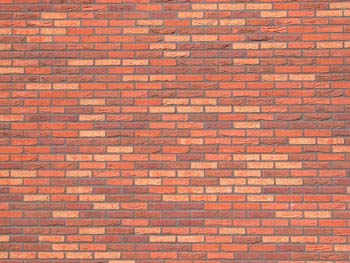
\includegraphics[width=0.8\textwidth]{../images/origin_.jpeg}
				\caption{墙面原图}
			\end{minipage}
			\begin{minipage}[t]{0.78\linewidth}
				\centering
				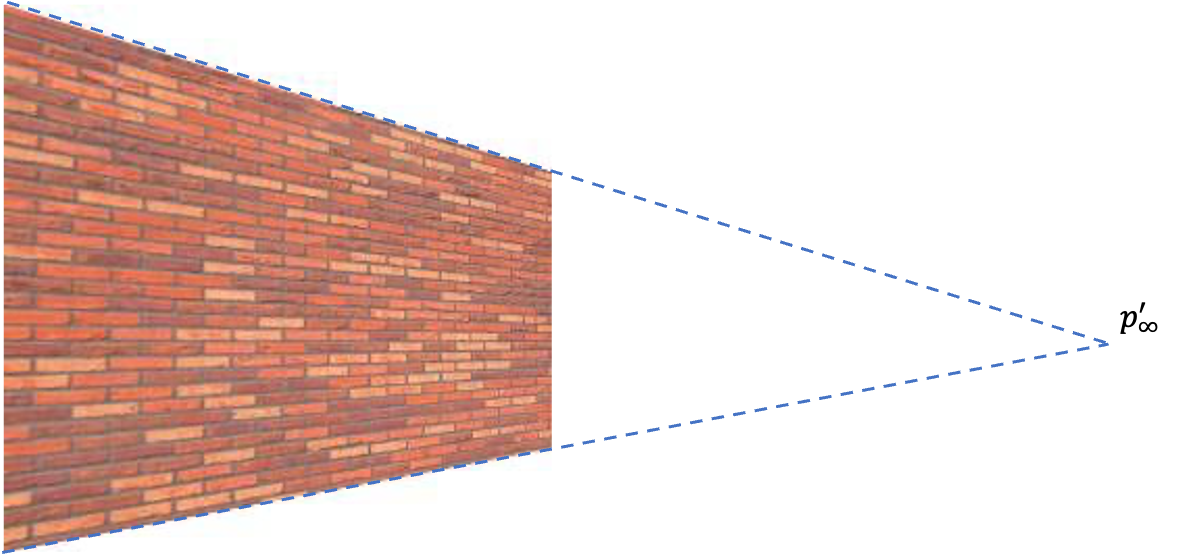
\includegraphics[width=0.8\textwidth]{../images/projective_.png}
				\caption{射影变换,无穷远点被映射为有限点}
			\end{minipage}			
		\end{figure}

		可以把无穷远点的像$p^{\prime}_{\infty}$映射回标准位置$(0,0,1)$,来恢复图像的仿射性质,具体来说,

		$$
			\mathbf{H}\mathbf{H_P}^{-1} = \mathbf{H_S}\mathbf{H_A}
		$$

		只要在图像上测量$p^{\prime}_{\infty}$的像素坐标,便可纠正图像的射影失真,恢复仿射性质,

		\begin{figure}[H]
			\begin{minipage}[t]{0.52\linewidth}
				\centering
				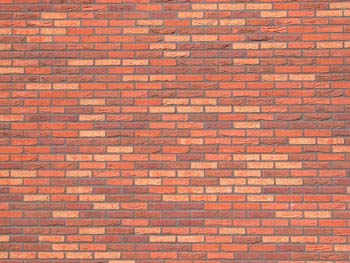
\includegraphics[width=0.8\textwidth]{../images/origin_.jpeg}
				\caption{墙面原图}
			\end{minipage}		
			\begin{minipage}[t]{0.5\linewidth}
				\centering
				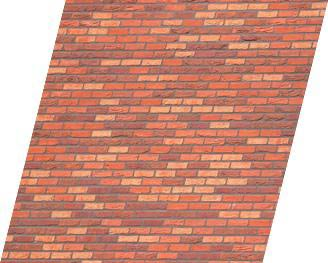
\includegraphics[width=0.8\textwidth]{../images/affine_.jpeg}
				\caption{仿射恢复,通过无穷远点消除射影失真}
			\end{minipage}			
		\end{figure}
		
		如果观察到更多的条件,可以继续消除仿射失真,恢复欧式性质。这就是变换的层次分解带来的好处。